% Options for packages loaded elsewhere
\PassOptionsToPackage{unicode}{hyperref}
\PassOptionsToPackage{hyphens}{url}
%
\documentclass[
  man,floatsintext]{apa6}
\usepackage{amsmath,amssymb}
\usepackage{iftex}
\ifPDFTeX
  \usepackage[T1]{fontenc}
  \usepackage[utf8]{inputenc}
  \usepackage{textcomp} % provide euro and other symbols
\else % if luatex or xetex
  \usepackage{unicode-math} % this also loads fontspec
  \defaultfontfeatures{Scale=MatchLowercase}
  \defaultfontfeatures[\rmfamily]{Ligatures=TeX,Scale=1}
\fi
\usepackage{lmodern}
\ifPDFTeX\else
  % xetex/luatex font selection
\fi
% Use upquote if available, for straight quotes in verbatim environments
\IfFileExists{upquote.sty}{\usepackage{upquote}}{}
\IfFileExists{microtype.sty}{% use microtype if available
  \usepackage[]{microtype}
  \UseMicrotypeSet[protrusion]{basicmath} % disable protrusion for tt fonts
}{}
\makeatletter
\@ifundefined{KOMAClassName}{% if non-KOMA class
  \IfFileExists{parskip.sty}{%
    \usepackage{parskip}
  }{% else
    \setlength{\parindent}{0pt}
    \setlength{\parskip}{6pt plus 2pt minus 1pt}}
}{% if KOMA class
  \KOMAoptions{parskip=half}}
\makeatother
\usepackage{xcolor}
\usepackage{graphicx}
\makeatletter
\def\maxwidth{\ifdim\Gin@nat@width>\linewidth\linewidth\else\Gin@nat@width\fi}
\def\maxheight{\ifdim\Gin@nat@height>\textheight\textheight\else\Gin@nat@height\fi}
\makeatother
% Scale images if necessary, so that they will not overflow the page
% margins by default, and it is still possible to overwrite the defaults
% using explicit options in \includegraphics[width, height, ...]{}
\setkeys{Gin}{width=\maxwidth,height=\maxheight,keepaspectratio}
% Set default figure placement to htbp
\makeatletter
\def\fps@figure{htbp}
\makeatother
\setlength{\emergencystretch}{3em} % prevent overfull lines
\providecommand{\tightlist}{%
  \setlength{\itemsep}{0pt}\setlength{\parskip}{0pt}}
\setcounter{secnumdepth}{-\maxdimen} % remove section numbering
% Make \paragraph and \subparagraph free-standing
\makeatletter
\ifx\paragraph\undefined\else
  \let\oldparagraph\paragraph
  \renewcommand{\paragraph}{
    \@ifstar
      \xxxParagraphStar
      \xxxParagraphNoStar
  }
  \newcommand{\xxxParagraphStar}[1]{\oldparagraph*{#1}\mbox{}}
  \newcommand{\xxxParagraphNoStar}[1]{\oldparagraph{#1}\mbox{}}
\fi
\ifx\subparagraph\undefined\else
  \let\oldsubparagraph\subparagraph
  \renewcommand{\subparagraph}{
    \@ifstar
      \xxxSubParagraphStar
      \xxxSubParagraphNoStar
  }
  \newcommand{\xxxSubParagraphStar}[1]{\oldsubparagraph*{#1}\mbox{}}
  \newcommand{\xxxSubParagraphNoStar}[1]{\oldsubparagraph{#1}\mbox{}}
\fi
\makeatother
\ifLuaTeX
\usepackage[bidi=basic]{babel}
\else
\usepackage[bidi=default]{babel}
\fi
\babelprovide[main,import]{english}
% get rid of language-specific shorthands (see #6817):
\let\LanguageShortHands\languageshorthands
\def\languageshorthands#1{}
% Manuscript styling
\usepackage{upgreek}
\captionsetup{font=singlespacing,justification=justified}

% Table formatting
\usepackage{longtable}
\usepackage{lscape}
% \usepackage[counterclockwise]{rotating}   % Landscape page setup for large tables
\usepackage{multirow}		% Table styling
\usepackage{tabularx}		% Control Column width
\usepackage[flushleft]{threeparttable}	% Allows for three part tables with a specified notes section
\usepackage{threeparttablex}            % Lets threeparttable work with longtable

% Create new environments so endfloat can handle them
% \newenvironment{ltable}
%   {\begin{landscape}\centering\begin{threeparttable}}
%   {\end{threeparttable}\end{landscape}}
\newenvironment{lltable}{\begin{landscape}\centering\begin{ThreePartTable}}{\end{ThreePartTable}\end{landscape}}

% Enables adjusting longtable caption width to table width
% Solution found at http://golatex.de/longtable-mit-caption-so-breit-wie-die-tabelle-t15767.html
\makeatletter
\newcommand\LastLTentrywidth{1em}
\newlength\longtablewidth
\setlength{\longtablewidth}{1in}
\newcommand{\getlongtablewidth}{\begingroup \ifcsname LT@\roman{LT@tables}\endcsname \global\longtablewidth=0pt \renewcommand{\LT@entry}[2]{\global\advance\longtablewidth by ##2\relax\gdef\LastLTentrywidth{##2}}\@nameuse{LT@\roman{LT@tables}} \fi \endgroup}

% \setlength{\parindent}{0.5in}
% \setlength{\parskip}{0pt plus 0pt minus 0pt}

% Overwrite redefinition of paragraph and subparagraph by the default LaTeX template
% See https://github.com/crsh/papaja/issues/292
\makeatletter
\renewcommand{\paragraph}{\@startsection{paragraph}{4}{\parindent}%
  {0\baselineskip \@plus 0.2ex \@minus 0.2ex}%
  {-1em}%
  {\normalfont\normalsize\bfseries\itshape\typesectitle}}

\renewcommand{\subparagraph}[1]{\@startsection{subparagraph}{5}{1em}%
  {0\baselineskip \@plus 0.2ex \@minus 0.2ex}%
  {-\z@\relax}%
  {\normalfont\normalsize\itshape\hspace{\parindent}{#1}\textit{\addperi}}{\relax}}
\makeatother

\makeatletter
\usepackage{etoolbox}
\patchcmd{\maketitle}
  {\section{\normalfont\normalsize\abstractname}}
  {\section*{\normalfont\normalsize\abstractname}}
  {}{\typeout{Failed to patch abstract.}}
\patchcmd{\maketitle}
  {\section{\protect\normalfont{\@title}}}
  {\section*{\protect\normalfont{\@title}}}
  {}{\typeout{Failed to patch title.}}
\makeatother

\usepackage{xpatch}
\makeatletter
\xapptocmd\appendix
  {\xapptocmd\section
    {\addcontentsline{toc}{section}{\appendixname\ifoneappendix\else~\theappendix\fi: #1}}
    {}{\InnerPatchFailed}%
  }
{}{\PatchFailed}
\makeatother
\keywords{proficiency, morphosyntax, bilingualism, ERP\newline\indent Word count: 1325}
\usepackage{lineno}

\linenumbers
\usepackage{csquotes}
\ifLuaTeX
  \usepackage{selnolig}  % disable illegal ligatures
\fi
\usepackage{bookmark}
\IfFileExists{xurl.sty}{\usepackage{xurl}}{} % add URL line breaks if available
\urlstyle{same}
\hypersetup{
  pdftitle={Proficiency and L2 Spanish Morphosyntax: An ERP Study},
  pdfauthor={Alexander Rogers1},
  pdflang={en-EN},
  pdfkeywords={proficiency, morphosyntax, bilingualism, ERP},
  hidelinks,
  pdfcreator={LaTeX via pandoc}}

\title{Proficiency and L2 Spanish Morphosyntax: An ERP Study}
\author{Alexander Rogers\textsuperscript{1}}
\date{}


\shorttitle{Proficiency and ERPs}

\authornote{

Department of Spanish and Portuguese.

The authors made the following contributions. Alexander Rogers: Conceptualization, Writing - Original Draft Preparation, Writing - Review \& Editing.

Correspondence concerning this article should be addressed to Alexander Rogers, 15 Seminary Place, New Brunswick, NJ. E-mail: \href{mailto:alexander.rogers@rutgers.edu}{\nolinkurl{alexander.rogers@rutgers.edu}}

}

\affiliation{\vspace{0.5cm}\textsuperscript{1} Rutgers University, New Brunswick}

\abstract{%
Proficiency and morphosyntax processing have long been demonstrated to have a predictable relationship. As a learner of a second language gains proficiency, they process morphosyntactic content more quickly and with higher accuracy. This has been demonstrated with a variety of methodologies, including eye-tracking, self-paced reading, and EEG. Differences in the amplitude and latency of the P600 ERP, commonly associated with morphosyntactic processing, have been found to correlate strongly with learner proficiency. What has not been found yet is whether these amplitude and latency differences can be utilized, in turn, to predict the proficiency of the learners. This study aims to fill that gap.
Our results show that this undertaking is more complicated than initially thought. Due to the nature of the data and the analytical methods used in this paper, the models were unable to predict proficiency. Perhaps with a different approach or with more experience this will succeed in a future endeavor.
}



\begin{document}
\maketitle

\section{Methods}\label{methods}

\subsection{Participants}\label{participants}

There were 81 (f = 55) participants in this study. Participants were from two possible language backgrounds: L1 Spanish monolinguals (n = 24) and L1 English learners of Spanish (n = 57). The learner participants were divided by proficiency level, including beginner (n = 11) intermediate (n = 11) and advanced (n = 25). All participants were recruited from either universities in the US (L1 English) or in Spain, Bolivia, and Paraguay (monolinguals).

\subsection{Material}\label{material}

Participants were assessed for proficiency level using a combination of two tests. First they completed the MLA Cooperative Language Test (Spanish Embassy, USA), then they completed the Cloze test from the DELE (Educational Testing Services, Princeton, USA). Following the proficiency tests, they completed the Language and Social Background Questionnaire (Anderson et al., 2019).

\subsection{Procedure}\label{procedure}

The study was conducted in two sessions: the first session was to complete the psychometric assessments and the background questionnaire. The second session was the EEG recording. In the EEG recording, they read sentences in three conditions one word at a time, and then completed a grammaticality judgement task after each sentence. The three conditions were ``grammatical'', ``gender violation'', and ``number violation''. There were 120 total stimuli, with 40 per condition. They were presented to the participants in a randomized, counterbalanced sequence in 6 blocks of 20.

\subsection{Data analysis}\label{data-analysis}

In this paper we attempt a novel analysis of data from a 2018 study by Aleman Banon et al.~The dataset contains datapoints for proficiency level (novice-advanced), proficiency test score (numeric), and the mean peak amplitude for each of 32 electrodes for each condition and time window. Before analysis, we tidied the data. The first step in the data tidying process was to isolate the electrodes from the central posterior region of the scalp (electrodes CP3, CPz, CP4, P3, Pz, P4, O1, Oz, O2) as that is the region suitable for characterizing the P600 ERP, which is most commonly associated with morphosyntactic processing. Once the electrode region of interest was isolated, we calculated the grand mean peak amplitude for that region for the three conditions: grammatical, number violation, and gender violation. The resulting dataset contains the aforementioned proficiency information as well as three data points per participant, their grand mean peak amplitude for each condition.
Once the data was properly tidied, we ran a series of nested model comparisons to evaluate the best fit model for the data. Because the scale of proficiency score and mean amplitude is so vastly different, we transformed the `mean' column by scaling it. The models were linear mixed effects models with proficiency as the target variable and the mean amplitudes as the predictor variables, with participant included as a random effect. This allows us to analyze the relationship between proficiency and ERP amplitude while allowing for the individual-level variation. While typical ERP research primarily makes use of ANOVAs and t-tests, we elected this novel form of analysis in an effort to try something new with the data.

\section{Results and Discussion}\label{results-and-discussion}

Figure 1 alloes us to visualize the overall trends in the data and to understand the relationship between our target and predictor variables before introducing the models.

\begin{figure}[H]
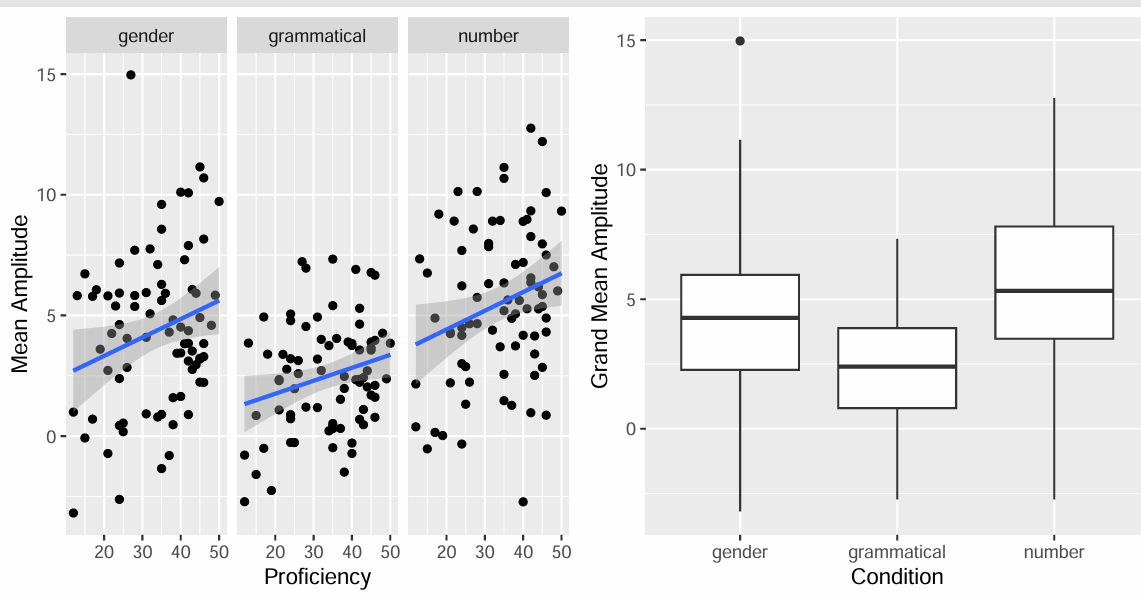
\includegraphics[width=\linewidth]{figs/plots} \caption{Amplitude by proficiency score and condition}\label{fig:fig-plots}
\end{figure}

Looking at the figures, we can see the generally expected outcomes. The amplitudes for the grammatical condition are the lowest, indicating that there was less neural activation in response to a sentence containing no erroneous content. This is to be expected, as the P600 ERP is typically only elicited by morphosyntactic violations. What is surprising, however, is that between the two violation conditions number violation had the higher overall peak amplitude. Since both English and Spanish mark plurals in the same way by utilizing inflectional morphology, but English does not have grammatical gender at all, it was predicted that the gender violation condition would haave the highest peak amplitude. Perhaps this can be attributed to the fact that English, while sharing the inflectional morphology for plural marking, does not necessarily have number agreement, and thus there necessitated some level of feature reassembly (Lardiere, 2009) caused by the cross-linguistic transfer. If the two structures are similar but not the exact same between languages, it is possible that this dissonance caused a processing delay.
Continuing to look at the plots, we can tell from figure 1 that the anticipated proficiency trend is in fact present. For each condition, as proficiency increased so too did the amplitude, demonstrating that more proficieny L2 learners of Spanish are more sensitive to grammatical violations and have an earlier and stronger ERP elicited in response to them, contributing to more ease in processing the L2.

\begin{verbatim}
## Data: df
## Models:
## mod_null: PROFICIENCY.TEST.SCORE ~ 1 + mean_scaled + (1 | PARTICIPANT)
## mod_2: PROFICIENCY.TEST.SCORE ~ 1 + mean_scaled + condition + (1 | PARTICIPANT)
## mod_3: PROFICIENCY.TEST.SCORE ~ 1 + mean_scaled + condition + (1 + mean | PARTICIPANT)
##          npar     AIC     BIC logLik -2*log(L)  Chisq Df Pr(>Chisq)    
## mod_null    4 -3194.8 -3180.9 1601.4   -3202.8                         
## mod_2       6 -3252.0 -3231.3 1632.0   -3264.0 61.261  2  4.983e-14 ***
## mod_3       8 -2096.3 -2068.6 1056.1   -2112.3  0.000  2          1    
## ---
## Signif. codes:  0 '***' 0.001 '**' 0.01 '*' 0.05 '.' 0.1 ' ' 1
\end{verbatim}

The nested model comparison run on the models demonstrated that the model utilizing mean and condition as predictors with a random intercept for participant was the best fir for the data with a p value of \textgreater0.001. The initial models were run using the non-scaled mean values, but repeatedly returned error messages. Thus, the current models were designed using the scaled means. The results changed very little, but the error messages disappeared. The detailed results of that model can be seen below.

\begin{figure}[H]
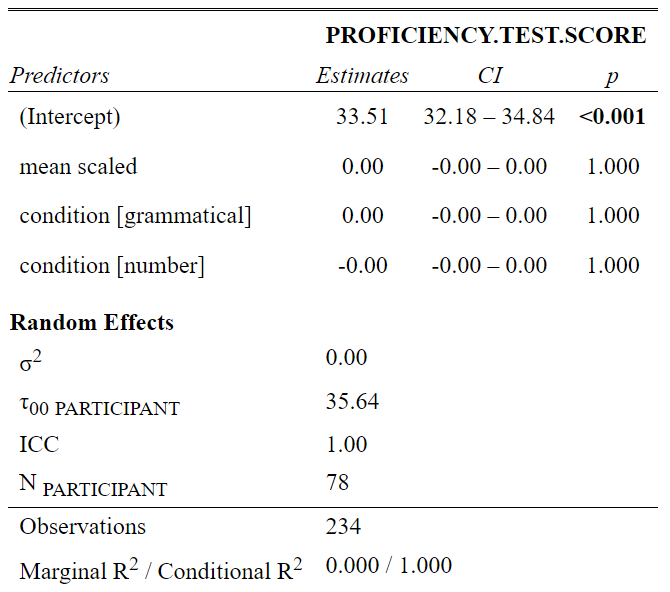
\includegraphics[width=\linewidth]{figs/mod_tab} \caption{Model summary}\label{fig:fig-mod-tab}
\end{figure}

The table summarizing our model demonstrates that it is not an ideal model design. While the intercept has a strong p-value, the rest do not. The intercept tells us that, for the gender violation condition, each 1-unit increase in mean peak amplitude for the P600 results in an increase of 33.51 points on a proficiency score. This is not very informative, as a 33 point increase is would nearly double a majority of scores, which is not a realistic outcome, and furthermore the amplitudes are typically below 1, so this is not very informative. Even using the scaled mean amplitudes the model gives us this outcome.

Based on my (limited) domain expertise ad well as looking deeper into this issue, it appears that the general idea of using proficiency score as a predictor is not very viable with the resources and knowledge available to me. Since each participant has a single proficiency score, there is no realistic way to assess the variance in that variable across conditions or means. While it would be relatively straightforward to adapt our analysis and utilize a different target variable (i.e.~mean) that does vary per participant per condition, that was not the goal of this project. The capacity to use proficiency as a predictor rather than target variable is well-established, and the purpose of this project was to attempt something novel. It is possible that this analysis can be done utilizing statistical or analytical methods that are outside of my current capabilities.

At the end of the day, there is a reason that the vast majority of ERP studies do not run models of this sort on the data, and simply conduct ANOVAs and t-tests as their primary methods of analysis. Linear models did not work with what I attempted to do, generalized linear models did not work particularly well, and mixed effects models also did not appear to work. It is possible to conduct a linear model if condition is taken out of the equation, but that leaves a single data point per participant and no real ability to compare between morphosyntax violation and grammatical, much less different types of violations as we have in this data. Moving forward, perhaps I will stick with self-paced reading and not go through the hassle of ERP data.


\end{document}
